\section{Print Controls}

\subsection{Approach}
There are many ways to create an FDM 3D printer, as seen in the many models available on the market, from industry-serving companies like Stratasys\footnote{\url{http://www.stratasys.com/}} and 3D Systems\footnote{\url{http://www.3dsystems.com/}} to home printer startups like Makerbot\footnote{\url{http://www.makerbot.com/}} to the many open-source efforts, notably the RepRap\footnote{\url{http://reprap.org/}} ecosystem. Most of these printers operate on Cartesian-style gantry system with 3 degrees of freedom. Some curved-layer printing is attainable on such printers, but the fixed attitude of the print heads limits the layer geometries to those that are accessible from one approach angle. To get around this limitation, a 6-degree-of-freedom robotic arm from FANUC\footnote{\url{http://www.fanucamerica.com/}} was used for this project. In addition to providing the 6 degrees of freedom necessary for curved-layer printing, the robot also provides 0.02mm of positioning repeatibility, which is small with respect to typical FDM nozzle outlet diameters (0.2-0.4mm). The robot was purchased in 2010 in the iRVision package as part of the CERT Program from FANUC. See the program brochure in Section~\ref{sec:cert-brochure} for more details.

Once the robot was chosen as the printing platform, much of the remaining 3D printing toolchain was filled in with parts and software from the RepRap community. These included the extruder hot-end and some related control hardware and software. Some additional control components were purchased from FANUC or fabricated in-house.

\subsection{Overview}
Figure~\ref{fig:sys-overview} gives a schematic overview of the mechanical, hardware, and software components that make up the curved-layer 3D printer system. The robot arm is the mechanical platform for the 3D printer. The custom extruder is fitted to the end of the robot arm and acts as a printing end effector. The motion of the robot arm is controlled by the robot controller, which is programmed by writing TP programs via the controller teach pendant. The extruder hardware, including the heater cartridge, cooling fan, and extrusion motor are controlled by an open-source Megatronics board loaded with the (also open-source) Marlin\footnote{\url{http://reprap.org/wiki/Marlin}} firmware. 

Normally, the Megatronics board is used to control the path of the extruder as well as the extrusion feed rate; the Marlin firmware can thus adjust the extruder filament feedrate according to the surface speed of the extruder in order to maintain the desired volumetric flow rate of hot plastic. However, in this case, the extruder path is controlled by the robot controller, so the extrusion control is independent of the motion control. Ideally, the two systems would be interfaced to allow the robot controller to give look-ahead speed predictions to the extruder controller to allow for tight synchronization. However, the FANUC controller interface only allows such interfacing with approved machinery. The next best option was to add I/O hardware to the FANUC controller and output an analog robot speed signal to the extruder controller. This way, the extruder controller might be able to extrude filament reasonably close to the actual extruder speed by tracking the robot speed output.

\begin{figure}
    \centering
    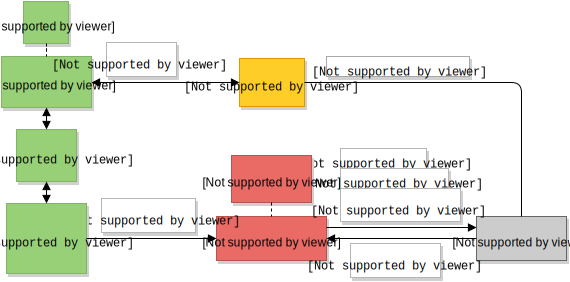
\includegraphics[width=.8\linewidth]{figures/diagrams/system overview}
    \caption{Overview of the 3D printer controls}
    \label{fig:sys-overview}
\end{figure}


\subsection{FANUC I/O interface}
    \subsubsection{Modules}
    \subsubsection{Housing design}
    \subsubsection{Wiring and connections}
\subsection{Jameco power supply}
\subsection{Megatronics board}
    \subsubsection{Mounting}
    \subsubsection{Wiring and connections}
    \subsubsection{Firmware}
